\documentclass{base}
\usepackage{hyperref}
\usepackage{array}

\renewcommand{\baselinestretch}{0.9}
\pagestyle{empty}
\begin{document}
\begin{center}
\begin{tabular}{>{\centering\arraybackslash}m{3cm}>{\centering\arraybackslash}m{10cm}}
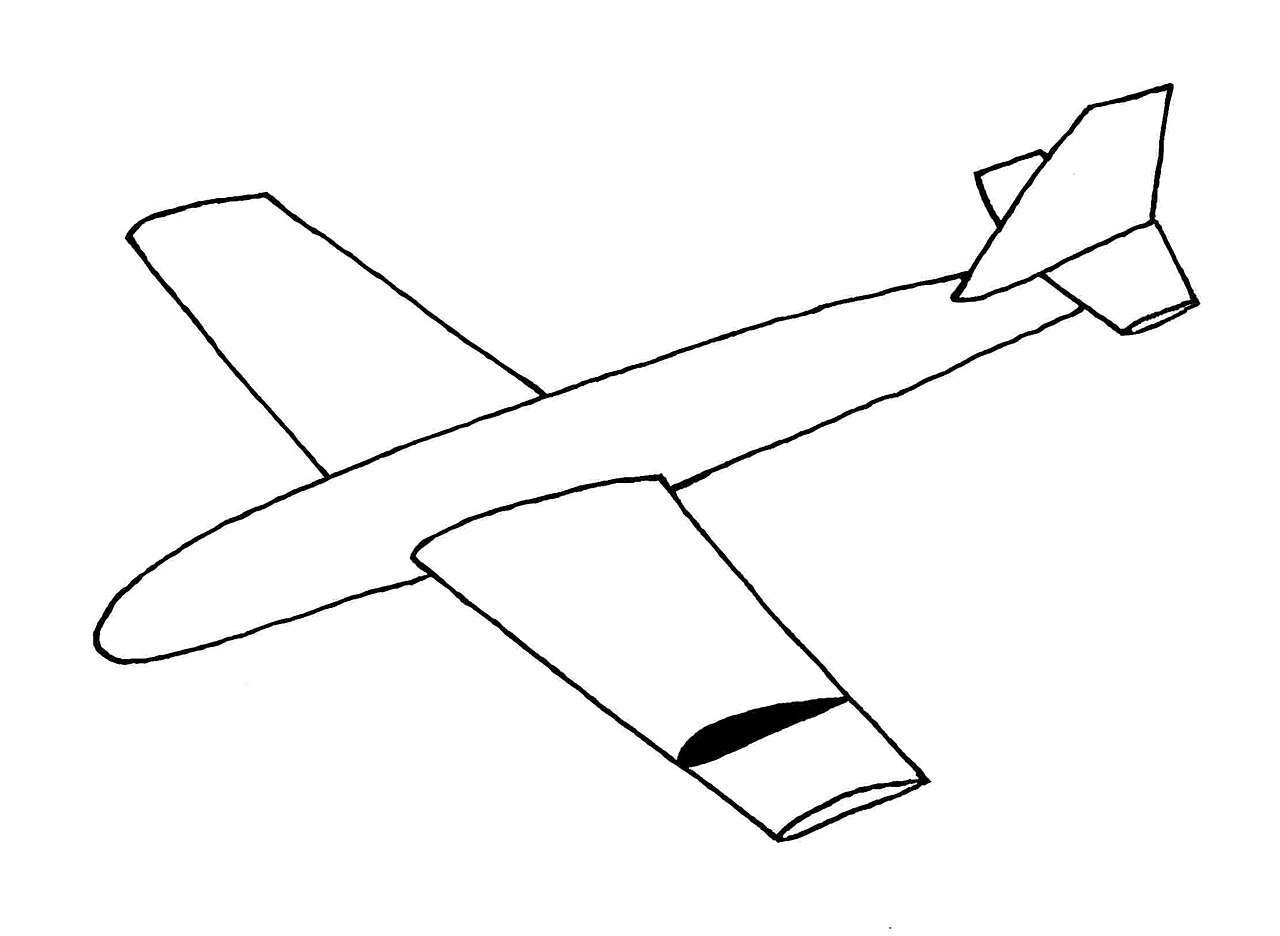
\includegraphics[width=\linewidth]{figures/introduction.jpg} & \Large \bf ENSTA Project - Exploring Airfoils Aerodynamics and Mechanics with Scientific Python\\
\end{tabular}
\end{center}

This project introduces scientific computing with Python through the study of some problems
in aerodynamics and flight mechanics. \textbf{No prior knowledge of these topics is assumed}.\\

The first part focuses on the prediction of the aerodynamic forces acting on an airfoil,
with particular emphasis on lift, drag, angle of attack,
and aerodynamic polars. Different modelling approaches will be investigated,
ranging from analytical models to semi-analytical and numerical methods,
and their predictions will be compared with experimental measurements\footnote{\url{https://m-selig.ae.illinois.edu/uiuc\_lsat.html}}.\\

Several classical aerodynamic tools will be implemented from scratch.
Among them, the Joukowsky transformation\footnote{\url{https://en.wikipedia.org/wiki/Joukowsky\_transform}}
will be used to generate and analyse airfoil geometries.
The results will then be analysed and compared with experimental data.\\

This part provides an introduction to the main principles of scientific programming:
translating physical and mathematical models into algorithms,
manipulating vectors and matrices with \texttt{\href{https://numpy.org/}{numpy}}, defining reusable functions,
performing numerical calculations.\\

The second part extends these models to flight mechanics, where the aerodynamic forces
are used to describe the motion and performance of an aircraft.
Several optimisation problems will be considered.
Numerical optimisation will be introduced through the discretisation of the control variables,
the definition of objective functions and constraints, and the use of appropriate optimisation tools
in the \texttt{\href{https://scipy.org/}{scipy}} library.\\


\begin{figure}[!h]
\centering
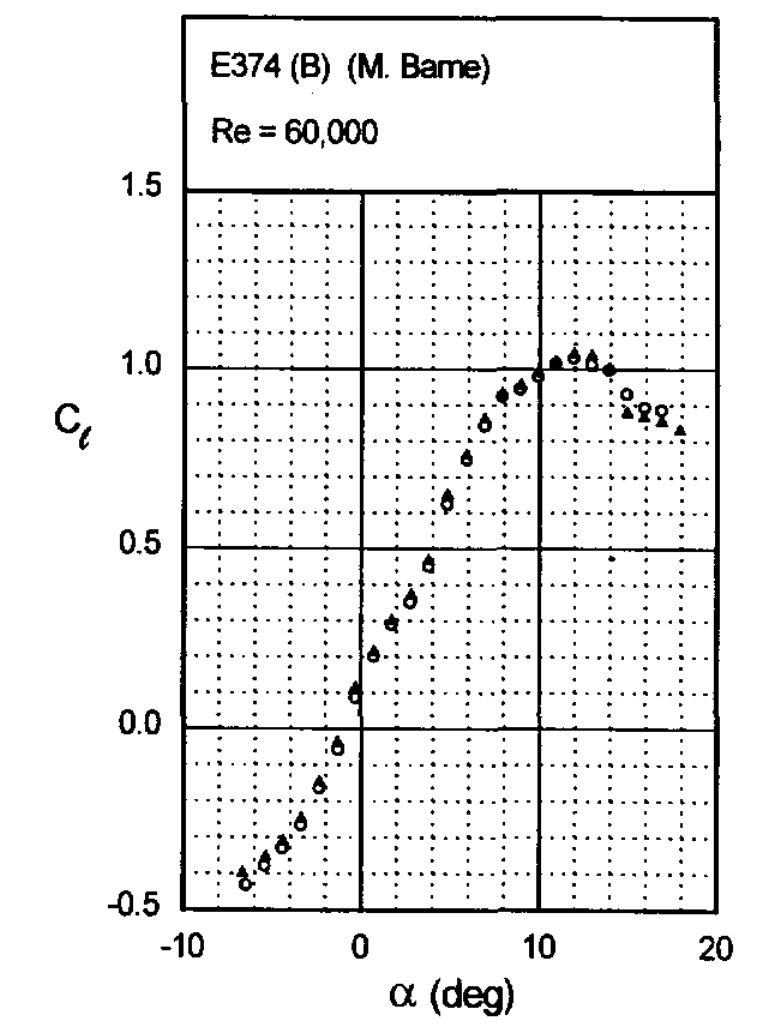
\includegraphics[width=0.3\textwidth]{figures/lift_curve.jpg}
\caption{E374 airfoil Lift evolution with respect to the angle of attack - Source:
\href{https://m-selig.ae.illinois.edu/uiuc\_lsat/Low-Speed-Airfoil-Data-V2.pdf}{Selig et al}}
\end{figure}

Throughout the project, scientific visualisation through a heavy usage
of the \texttt{\href{https://matplotlib.org/}{matplotlib}} and \texttt{\href{https://pandas.pydata.org/}{pandas}} libraries will play a central role:
airfoil geometries\footnote{\url{https://m-selig.ae.illinois.edu/ads/coord\_database.html}},
flows, aerodynamic polars, trajectories, and more will be represented using Python.
The focus will be placed not only on obtaining numerical results, but also on visualising,
comparing and validating computational predictions.


\end{document}